\documentclass[11pt]{article}

\usepackage[margin=1.25in]{geometry}

\usepackage{amsmath}
\usepackage{amssymb}
\usepackage{graphicx}
\usepackage{amsfonts}
\usepackage{dutchcal}
\usepackage{braket}
\usepackage{enumitem}

\usepackage{tikz}
\usepackage{forest}
\usetikzlibrary{trees}
\usetikzlibrary{calc}
\usepackage{calculator}
\usepackage{standalone}



\begin{document}

\title{Hamiltonian mechanics is conservation of information entropy}
\author{Gabriele Carcassi, Christine A. Aidala}


%\ifjournal
%	% As the page margins are so large, the full title does not fit
%	\titlerunning{From physical principles to classical and quantum particle mechanics}
%\fi

\date{\today}

\maketitle

\begin{abstract}
	In this work we show the equivalence between Hamiltonian mechanics and conservation of information entropy. We will show that distributions with coordinate independent values for information entropy require that the manifold on which the distribution is defined is charted by conjugate pairs (i.e. it is a symplectic manifold). We will also show that further requiring that the information entropy is conserved during the evolution yields Hamilton's equations.
\end{abstract}

\tableofcontents
\newpage

\section{Introduction}

Over the past decade there has been a renewed interest in the underpinning of classical mechanics. Different attempts and arguments have been put forward to understand what are the most important features of the various mathematical formulations, whether they are equivalent or whether one is more fundamental than the other~\cite{North,Curiel,Barrett1,Barrett2}. We believe, though, that there are two general problems with these attempts.

The first is that they concentrate on the mathematical structure which, unfortunately, is not enough to characterize a physical theory. They all note how the same physical system can be described by different mathematical frameworks. For example, a classical system can be characterized by position and velocity in the Lagrangian framework and by position and momentum in the Hamiltonian framework. They do not note, though, that the converse is also true: the same mathematical equation can represent two different physical systems. For example, the equation $ma + bv = 0$ in the context of Newtonian mechanics can either represent a body in an inertial frame under linear drag or a body in a non-inertial frame with no forces acting on it. If $t_{in}$ is time in the inertial frame, the time $t$ in the non-inertial frame is such that  $\frac{dt}{dt_{in}} = e^{\frac{b}{m}t}$. Mathematical equivalence does not imply physical equivalence, which is especially problematic for \cite{Barrett2} since it focuses on the former. In other words, we can have the same physics with different math and the same math with different physics. The connection between math and physics is many-to-many because mathematics captures only the syntax of a particular description without its semantics, which at that point cannot be recovered.

As we do not have a one-to-one map between math and physics, fixating on the mathematical structure may even confuse us. For example, it is known\cite{AllHamFreeParticle} that any Hamiltonian system is, at least locally, equivalent to a free particle. That is, we can always find a canonical transformation (i.e. a transformation that does not change the equation of motion) such that any Hamiltonian system, in the new coordinates, has the motion of a free particle for a finite amount of time. As \cite{North} notes, only frame-independent relationships should be taken as fundamental. Does that mean that the Hamiltonian itself is not fundamental because it is not invariant under canonical transformations? Does it mean that all Hamiltonian systems are the same system, since there is always a set of canonical coordinates in which $H=p^2/2m$? It is also known\cite{AllSystemsAreHam} that for any first-order system of ordinary differential equations we can find an appropriate symplectic structure such that the system can be written as a Hamiltonian system. Does that mean that, in the end, all systems are physically equivalent, regardless of what they describe? The point is, we cannot know whether our findings about mathematical structures are physically significant if we do not have a precise link between the mathematical symbols and their physical meaning.

This leads us to the second problem we believe the previous works may have: when trying to attach meaning the thinking and intuition is still Newtonian. This is particularly evident in \cite{Curiel} where physical ideas provide the starting point to get to Lagrangian dynamics. The starting point is that a classical system is one that, roughly, obeys Newton's second law and therefore we have, for a free particle, $\dot{x} = v$ and $\dot{v} = 0$. Unfortunately this is only true in an inertial frame. As \cite{North} notes, both Hamiltonian and Lagrangian mechanics are coordinate independent: the equations are valid in all reference frames even non-inertial ones. In fact, that is probably the most notable advantage of the frameworks, that fictitious forces are automatically handled. But none of the Newtonian concepts are coordinate independent: inertial frames, absence of forces and even conservation of energy are all frame dependent. This, again, leads to confusion and we may miss a key element: in the transition from Newtonian to Lagrangian/Hamiltonian mechanics we expand the reference frames in which the equations are valid (from inertial frames to all frames) at the expense of restricting the class of systems we can describe (e.g. dissipative forces in general require a modification of the Euler-Lagrange equation typically using the Rayleigh dissipation function). The point is, Newtonian concepts may prevent us from fully understanding Hamiltonian and Lagrangian mechanics.

It should be clear that we do not fault the authors. We fault ourselves, the physicists. Even just a century ago, there was a push in our field to find fundamental principles or laws that could serve as a starting point for the different theories. Newtonian mechanics, thermodynamics and special relativity serve as good examples. Nowadays, unfortunately, many of the current fundamental theories, including Lagrangian, Hamiltonian, quantum mechanics and quantum field theory take as their starting point a particular mathematical structure. That is, we do not know what the value of a Lagrangian means or what the symplectic form represents; we just take them as given. Moreover, a lot of work in theoretical physics nowadays starts by exploring novel abstract mathematical structures and then trying to see whether some physical meaning or prediction can be extracted. We are not going to debate here how and why this shift happened. We merely note that it leaves the semantics of our theories ill defined.\footnote{Which is a nice way to say that we don't really know what we are talking about.} 

It is only natural that, given the circumstances, a philosopher would use the only thing that seems to be well defined, the math, and try to draw understanding from there. But here lies the fundamental problem: that math is not created by physicists to do physics, it is created by mathematicians to do math. The definitions of topology, differentiable manifold, symplectic manifold, Hilbert space and so on are chosen either because they are convenient to prove theorems or because they are convenient to perform calculations.\footnote{In fact, it is common in math to have two such definitions and then prove they are equivalent.} We should not expect them to be a good match for definitions that would be physically meaningful. In other words, there is a very good chance that looking at just the math may lead us, like horses with blinders, in a well-defined direction which is not the physically meaningful one. To be clear, we do not fault the mathematicians either as they are not responsible for whether their structures are used appropriately or not within physics.

As all these problems stem from a lack of physical principles that can serve as a foundation for classical Hamiltonian and Lagrangian mechanics, we turn to a recently published work\cite{AoPPhy1} that aims to identify such starting points. Inspired by those insights, we fully develop another that is only briefly hinted at in that work: the idea that \textbf{a distribution over a manifold conserves information entropy over time if and only if its elements evolve according to Hamiltonian mechanics.} That is, the single requirement of information entropy conservation not only gives us Hamiltonian dynamics but also the structure of phase space (i.e. a symplectic structure where variables are organized in conjugate pairs).

We believe this insight may be of interest to the philosophy of science community for at least two reasons. First because it helps to clearly characterize what Hamiltonian mechanics describes, providing a clear physical meaning to the mathematical structures used. This should be at least of interest to that part of the philosophy community interested in the foundations of classical mechanics. Second because information entropy has a deep connection to the foundations of thermodynamics, therefore the strong link we establish here between information entropy and Hamiltonian mechanics should be of interest to an even wider audience.

We begin in section 2 by giving a brief summary of statistical distributions in general. These are your typical mathematical tools used to keep track of how charge is distributed in space or how a population of individuals is distributed in age. We briefly introduce information entropy, which measures the number of yes or no questions one has to answer to be able to identify a particular element within a distribution. The main issue is that the density and the information entropy for a distribution depend, in general, on the variables and their units. For example, if we change our units from meters to kilometers a density of $1 kg/m^3$ would change to $10^9 kg/km^3$. In other words, distributions are not in general invariant under change of variables. In section 3 we look at distributions over states. We argue that since states themselves are coordinate independent, the density and information entropy associated with them cannot be coordinate dependent. Moreover, a deterministic and reversible system must be one that preserves information entropy over time (i.e. information about the system at one time is equivalent to information about the system before or after). The requirement of coordinate-independent distributions gives us the symplectic structure (i.e. conjugate pairs of position and momentum) while the requirement of conservation of information entropy gives us Hamiltonian evolution. In section 4 we discuss the result and provide a dictionary that allows us to give precise meaning to the different mathematical symbols, addressing the issues highlighted before. We also show how this understanding allows us to construct a classical analogue of the uncertainty principle.

\section{Distributions}

Our starting point is the standard concept of a statistical distribution. We have a set of elements, also called population, and a set of variables that characterize some properties of those elements. To each element is associated a value for each variable and we want to describe how the population is distributed over the possible values of the variables. For example, people by age and country of residence, amount of material among different compounds, mass or charge over different positions in space. In all these cases, we have a total quantity $M$ that measures how many elements we have. This can be either a discrete quantity, like the number of people we are considering, or a continuous quantity, like the total amount of mass. We also have a set of $n$ variables $\xi^a$ over which the elements are distributed and a function $m(\xi^a)$ that gives us the amount for each value possible value such that:
\begin{equation}
\int m(\xi^a) d\xi^1 d\xi^2 ... d\xi^n = M
\end{equation}
The integral is used when some of the variables $\xi^a$ are continuous, and a simple sum would be used over the discrete ones. We can also define the normalized density as:
\begin{equation}
\rho(\xi^a) = \frac{1}{M}m(\xi^a)
\end{equation}
To calculate the amount in a particular region $V$ we have:
\begin{equation}
m_V = \int_V M \rho(\xi^a) d\xi^1 d\xi^2 ... d\xi^n
\end{equation}
The above expression would represent the mass or charge within a particular region, the amount of material of some selected set of compounds or the world population in a particular set of countries and age group. We can also define:
\begin{equation}
\mu(V) =\frac{m_V}{M} = \int_V \rho(\xi^a) d\xi^1 d\xi^2 ... d\xi^n \\
\end{equation}
which gives the fraction of the population within that region.

The normalized distribution $\rho(\xi^a)$, as defined, is a statistical distribution that represents the entirety of the system being described. Yet, we can give it an additional meaning of probability if we run the following thought experiment: suppose we took an element at random, each element with equal chance, what is the probability $P(\xi^a \in V)$ that the values for $\xi^a$ associated with that element are within a particular region $V$? The answer must be $\mu(V)$ and therefore $\rho(\xi^a)$ is the probability density. So $\rho(\xi^a)$ has this double role as a physical statistical distribution and a conceptual probability distribution for our thought experiment. This second role is our link to information theory.

Before proceeding, though, let us give a quick introduction so that we have a clear understanding about what information entropy represents. In the physics community, for example, the concept is often vaguely referred to as ``knowledge" (and sometimes as ``lack of knowledge") which is incorrect and misleading.\footnote{We believe this characterization may be due to Jaynes\cite{Jaynes} who first introduced the concept of information theory within thermodynamics. Note that we are only going to talk about information entropy and not thermodynamic entropy. We do believe there is a link between the two, but it is not the one Jaynes gives. We leave that discussion for another work.} Information entropy was introduced by Shannon\cite{Shannon} to solve specific engineering problems and therefore, like distance or mass, information entropy is a number that measures a well defined quantity and should be treated as such. What he needed was a way to measure how much information a particular channel is able to transfer and therefore a way to quantify precisely information as number of bits. So the idea is that we have a source that sends messages to a destination, and the message is encoded in zeros and ones. Information entropy is the optimal average number of zeros and ones that must be used to encode the messages. A message with fewer bits is crippled, and a message with more bits is redundant.

To understand how this works in our context, let us go back to our distribution $\rho(\xi^a)$ and refine our thought experiment. Suppose two individuals, Alice and Bob, have full knowledge of the same distribution. Suppose Alice picks an element at random and Bob needs to know the value of the variable for the element Alice picked. That is, Alice is the source, Bob is the destination and the message is the value of the element Alice picked from the distribution. How long, on average, should the message be? How many ones and zeros? How many yes or no questions must Bob ask Alice before he knows the value? For example, suppose there are 40 balls of which 20 are red and 20 are green. In that case one yes or no question (``Is it green?"), one bit of information, would be sufficient. Suppose there are 40 balls of which 10 red, 10 green, 10 blue and 10 yellow. In this case, two questions would suffice as shown in figure \ref{twoQuestions}, since two yes or no questions, two bits of information, can distinguish 4 cases.

\begin{figure}\label{twoQuestions}
	\centering
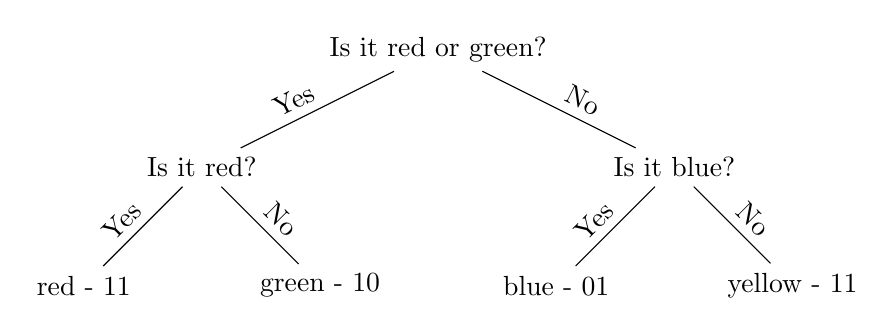
\begin{tikzpicture}[level distance=1.5cm,
level 1/.style={sibling distance=6cm},
level 2/.style={sibling distance=3cm}, sloped]
\node {Is it red or green?}
child {node {Is it red?}
	child {
		node {red - 11}
		edge from parent node[pos=0.6, align=center, above] {Yes}
	}
	child {
		node {green - 10}
		edge from parent node[pos=0.6, align=center, above] {No}
	}
	edge from parent node[pos=0.6, align=center, above] {Yes}
}
child {node {Is it blue?}
	child {
		node {blue - 01}
		edge from parent node[pos=0.6, align=center, above] {Yes}
	}
	child {
		node {yellow - 11}
		edge from parent node[pos=0.6, align=center, above] {No}
	}
	edge from parent node[pos=0.6, align=center, above] {No}
};
\end{tikzpicture}
\caption{The decision tree for the example in the text. The nodes of the tree represent the questions Bob can pose to Alice and the bottom line shows the four different cases with the corresponding encodings.}
\end{figure}


In general, if $I$ is the number of questions, the number of bits, then $C = 2 ^ I$ are the number of cases one can distinguish with those questions. On the other hand, suppose for a particular value $\xi_0$ of a discrete variable we have $\rho(\xi_0)=1/5$, then we know that we'd select $\xi_0$ one in 5 cases. That is, the normalized distribution is the inverse of the number of cases: $\rho(\xi_0) = \frac{1}{C}$.  Therefore the information needed to identify a particular case is $I(\xi^a)=\log \frac{1}{\rho(\xi^a)}$. If we take the average and change the base of the logarithm, we have:
\begin{equation}
I(\rho(\xi^a)) = \int \rho(\xi^a) \ln \left(\frac{1}{\rho(\xi^a)}\right) d\xi^1 d\xi^2 ... d\xi^n =-\int \rho(\xi^a) \ln (\rho(\xi^a) d\xi^1 d\xi^2 ... d\xi^n
\end{equation}
which is the information entropy of the distribution. That tells us the average number of bits one needs to put into a message to tell someone else the value of the element of the distribution that was picked at random.

Technically, given the more convenient choice of the natural logarithm, the unit of information is the nat, which is equal to $\frac{1}{\ln 2}$ bits. However, in the discussion we will refer to it as measured in bits, as we believe that the majority of the readers is more comfortable with the latter unit. Also, technically, for continuous variables the expression has a slightly different meaning: the uniform distribution in a unit volume is assigned zero entropy so $I(\rho(\xi^a))$ represents the relative number of bits to achieve the same level of precision, which can be negative. That is, if we take a real number from a uniform distribution between 0 and $\frac{1}{2}$ we need to lose a bit of information to get to the same precision of a unitary distribution.

Technicality aside, the above discussion, while not a formal derivation, should give a sense of what the expression signifies: it measures the \emph{additional} information that would be needed to identify the value associated to an element picked at random from a known population. What is also important is that it is a precisely defined quantity and that there is only one way to define it. It is the only expression that satisfies three simple requirements (continuity, monotonicity and additivity) that are necessary to measure information, and that is how Shannon originally derived it. Insofar that we want to talk about amounts of information we have only one way to do so.

\subsection*{Densities and change of variables}

There is one feature about densities we need to be fully aware of: in general they are not invariant under change of variables. Intuitively, if we change units the density changes value. For example, a linear mass density of $1$ kg/m at $20$ Celsius for one references becomes a linear density of $1000$ kg/km at $20$ Celsius. The temperature does not change value (it is a scalar and therefore invariant) while the density changes value. Physically, we use the unit to understand that the overall quantity is the same. But mathematics only keeps track of the number, which changes, and is therefore coordinate dependent. In general, if $\hat{\xi}^a=\hat{\xi}^a(\xi^b)$ we can recover how the density changes by requiring that the total in each volume is the same no matter what variables are used. That is:
\begin{align*}
\int_V \rho(\xi^b) d\xi^1 ... d\xi^n &= \int_V \rho(\hat{\xi}^a) d\hat{\xi}^1 ... d\hat{\xi}^n \\
&=\int_V\rho(\hat{\xi}^a) \left\|\frac{\partial \hat{\xi}^a}{\partial \xi^b}\right\| d\xi^1 ... d\xi^n
\end{align*}
\begin{equation}\label{density_transformation}
\rho(\xi^b) = \rho(\hat{\xi}^a) \left\|\frac{\partial \hat{\xi}^a}{\partial \xi^b}\right\|
\end{equation}
the density is multiplied by the absolute value of the Jacobian determinant of the transformation. As the Jacobian is in general a function of the variables themselves, this means that whether the density at one point is greater or smaller than at another also depends on the choice of variables.

Similarly, we can see that information entropy is not invariant
\begin{align*}
I(\rho(\xi^b)) &=-\int \rho(\xi^b) \ln (\rho(\xi^b)) d\xi^1 ... d\xi^n \\
&=-\int \rho(\hat{\xi}^a) \left\|\frac{\partial \hat{\xi}^a}{\partial \xi^b}\right\| \ln \left(\rho(\hat{\xi}^a) \left\|\frac{\partial \hat{\xi}^a}{\partial \xi^b}\right\|\right) d\xi^1 ... d\xi^n \\
&=-\int \rho(\hat{\xi}^a) \ln \left(\rho(\hat{\xi}^a) \left\|\frac{\partial \hat{\xi}^a}{\partial \xi^b}\right\|\right) d\hat{\xi}^1 ... d\hat{\xi}^n \\
&=-\int \rho(\hat{\xi}^a) \ln (\rho(\hat{\xi}^a)) d\hat{\xi}^1 ... d\hat{\xi}^n -\int \rho(\hat{\xi}^a) \ln \left\|\frac{\partial \hat{\xi}^a}{\partial \xi^b}\right\| d\hat{\xi}^1 ... d\hat{\xi}^n
\end{align*}
\begin{equation}\label{entropy_transformation}
I(\rho(\xi^b)) =I(\rho(\hat{\xi}^a)) -\int \rho(\hat{\xi}^a) \ln \left\|\frac{\partial \hat{\xi}^a}{\partial \xi^b}\right\| d\hat{\xi}^1 ... d\hat{\xi}^n
\end{equation}
The reason is that we may be changing scale and therefore level of precision required to describe our value. Given that the change in both density and entropy is determined by the Jacobian, we conclude that \textbf{during a change of variable the information entropy of all possible distributions does not change if and only if the density remains the same at every point under the same change of variable}.

To sum up, while we would like to think of a density as a number associated to a point of a space, that is technically incorrect. Given a manifold $\mathcal{M}$ upon which we define the distribution, the latter is \emph{not} $\rho : \mathcal{M} \to \mathbb{R}$ in general. That would be a scalar function, invariant under change of variables, as a point is a point no matter how it is identified. Instead we additionally need a set of functions $\xi^a : \mathcal{M} \to \mathbb{R}$ and only then we can define the density as $\rho : \mathbb{R}^n \to \mathbb{R}$. The density value is defined on the values for a set of variables, not at a point.\footnote{As the density is really a limit, we need to know how that limit is taken, and the coordinates decide that.} That is, the density is undefined without a (differentiable) set of coordinates.

\subsection*{Mathematical tools for distributions}

Different fields in math deal with the coordinate dependency of densities in different ways depending on their aims, which unfortunately leads to a fractured physical understanding given that one needs ideas and results from the different areas. In statistics and information theory one simply accepts the transformation rules and does not try to create invariant objects. This gives us the proper setting to study the statistical properties but it does not help us understand which mathematical elements represent objective physical entities.

In probability theory one starts with three objects: a set of outcomes $\mathcal{M}$, a set of events $\sigma_\mathcal{M}$ where each event is a collection of outcomes, and a probability measure $\mu : \sigma_\mathcal{M} \rightarrow [0,1]$ that assigns a number between zero and one to each event. That is, we do not assign a probability density to the points of $\mathcal{M}$ but we assign a finite probability to finite regions. We can then define a random variable $\xi : \mathcal{M} \rightarrow \mathbb{R}$ as a real-valued function of the outcomes. For each random variable we can define its cumulative distribution function $F_\xi(\xi_0)=\mu(\xi<\xi_0)$ and the probability density function is its Radon-–Nikodym derivative $\rho(\xi) = \frac{dF_\xi}{d\xi}$. That is, the integral is the primal object while the density is derived.

This approach, if applied to statistical distributions, actually makes more physical sense: what we measure is the amount of mass in a finite region and the density is the limit for a smaller and smaller one. The fundamental objects (outcomes, events and probability) are all defined without reference to variables. It also has the advantage that discrete and continuous quantities are treated in the same way. But in probability theory we have no notion of coordinate systems, vectors or any other geometrical objects.

In differential geometry, one starts with a manifold: a set of points $\mathcal{M}$ which can be given local coordinates $\xi^i : \mathcal{M} \to \mathbb{R}$. One defines a tangent space $\mathsf{T}\mathcal{M}$ where vectors live and cotangent space $\mathsf{T}^*\mathcal{M}$ were linear functions of vectors live. Then we define $n$-forms as multi-linear functions of $n$ vectors that return the value associated with the infinitesimal parallelepiped they form. That is $\nu : (\mathsf{T}\mathcal{M})^n \rightarrow \mathbb{R}$. As vectors are coordinate invariant, $n$-forms are coordinate invariant as well so we can write $\mu(V)=\int_V \nu$ with no reference to coordinates. If $e_a$ are the basis vectors associated with $\xi^a$ and $e^b$ are linear functions such that $e^b(e_a)=\delta_a^b$, then we can express each $n$-form as $\rho(\xi^a)e_1\wedge e_2 \wedge ... \wedge e_n$. The density $\rho(\xi^a)$ is the component of the $n$-form expressed in the $\xi^a$ coordinates in a way analogous to components of a vector.\footnote{Technically, the form is linear so it changes with the Jacobian determinant and not its absolute value. But a negative determinant means changing orientation of the region of integration, so fixing that would bring another sign change and $\rho(\xi^a)$ would not change. This is equivalent to saying that some coordinate systems are right handed and some are left handed.}

This approach gives us a way to understand which objects are coordinate independent and which are not. But it has two issues: it does not allow us to easily talk about coordinate dependent operations, such as marginal distributions and information entropy, and it may use definitions that do not map well to physical concepts. For example, a vector is typically defined as a map between a scalar function of the manifold to another scalar function of the manifold, or as an equivalence class of trajectories. It is a stretch to think of fluid velocities or electric fields in those terms.\footnote{For that same reason, we do not use the differential geometry notation $\frac{\partial}{\partial \xi^a}$ and $d\xi^a$ for vector and covector basis because they do not convey the actual physical meaning of these objects as they are used in physics. This is another instance of the math-for-mathematician issue.}

So the situation is that we have a single clear physical object we want to study, a statistical distribution, but different and somewhat disconnected mathematical frameworks to study it. As noted in the introduction, this should not be surprising as the frameworks are defined by mathematicians to solve their own needs. But it is an issue when these are used in physics without careful consideration, as each mathematical framework may only partially capture our physical understanding. And this is precisely why we argue that simply examining the mathematical structure used in a physical theory is not enough to gain a complete picture: mathematics can only check for self-consistency and not for completeness or correctness. What we will need to do, in fact, is use elements from all these frameworks as some insights are better understood in one context and some in another.

\section{Coordinate independent distributions}

We now turn our attention to what we call infinitesimally reducible systems: a system whose overall state can be reduced to the state of its infinitesimal parts. That is, we can think of our system as made of infinitesimal pieces, which we call particles. Each particle is in a state from a state space $\mathcal{S}$. The state of the whole system, then, will be described by a distribution $\rho : \mathcal{S} \to \mathbb{R}$ over those states. That is, the elements of our distributions are the particles, the variable associate to each element is the state of the particle. Here we have the first problem: states, to be physically objective, must be coordinate independent objects. We \emph{do} want the density to be define on the actual space $\mathcal{S}$ or our distribution would not be physically meaningful. But we said before that, in general, densities are defined on the state variables, not on the object the state variables identify.

Now suppose that this system evolves in a way that is deterministic and reversible, that is the state of a particle at one time is associated with one and only one state at another time. What does that tell us about our distribution? If the evolution is deterministic and reversible, then all the parts that are in one state will be mapped to another: the density should be exactly mapped to a different state and therefore should not change value. If the evolution is deterministic and reversible, then if I give you enough information to identify the state of an element at one time I also gave you enough information to identify the state of the same element at a future time: the information entropy will remain the same over time. And here lies another problem: how can we make sure that these quantities are preserved over time if they are not even observer independent? How can we know if the density stays the same if we can't even compare the value of the densities at two different elements of the distribution? How can we tell whether the information entropy is conserved if we can't even define a unique value at a given time?

We are forced to conclude that \textbf{if we want to define deterministic and reversible evolution over distributions, they must be invariant distributions. That is, the densities and information entropy must be independent of the choice of coordinates.} As we noted before, requiring one to be coordinate invariant will automatically require the other to be invariant as well. In other words, the state for an infinitesimally reducible system must be an invariant distribution over the states of the particles. 

If our variables are discrete, all our integrals are sums and all our definitions work. Everything is already coordinate invariant. If our variables are continuous, instead, we have a problem. Because the densities and the information entropy vary with the Jacobian, we need something more. Our state space $\mathcal{S}$ must allow us to write densities whose value does not change under coordinate transformation. That is, the density must be change with the Jacobian (i.e. something we can integrate on) but also not change at all (i.e. the number is coordinate independent). This seems to be impossible given what we saw before: how can it work?

Suppose $\mathcal{S}$ is a two dimensional manifold. Suppose we have two variables $(q,k)$ such that $k$ uses the inverse units of $q$. For example, if $q$ is meters then $k$ is inverse meters which means an infinitesimal area $dq dk$ will be a pure number. We say $q$ is a coordinate as it is a variable that defines a unit, while $k$ is the corresponding conjugate variable as it uses the inverse unit. Now suppose you change coordinate. For example, $\hat{q}$ will be kilometers and $\hat{k}$ inverse kilometers. We'll have $d\hat{q} d\hat{k} = dq dk$. Therefore we'll also have $\rho(q,k) = \rho(\hat{q}, \hat{k})$: the density is invariant and so is the information entropy.

Note how we have to separate the idea of state variables, a value used to identify a state, from a coordinate, a state variable that defines the system of units and references. The insight is that the link does not necessarily have to be one to one. One choice of coordinate can influence more then one state variables. But how many can it influence?

It turns out that if we have a set of variables fixed by a single choice of unit, a single coordinate, then what we discussed before is the only possible way. Let $q$ be the coordinate, the variable that defines the unit. Suppose we have $n$ variables $\xi^a$ such that $\xi^1 = q$. Each vector $v^a$ tangent to that space has $n$-components. If we change unit $\hat{q}=\hat{q}(q)$ we have two constraints: the one unit change and the unitary Jacobian, and these must be enough to determine how the vector components change. The number of components must be equal to the number of constraints and therefore there are exactly two variables $\xi^a = (q, k)$. Then $k$ is the conjungate variable of $q$.

Physically, the coordinate plays a double role. It both defines a unit and it helps identify particle states. It is this double role that gives it an important character because a change in $q$ must induce a change in $k$ as their units and the unit of $\rho$ are not independent. Symplectic geometry strips away the units and does not elevate densities as primary objects. It is no wonder the link gets lost. But that's what, ultimately, is describing.

\subsection*{Hamiltonian mechanics for one degree of freedom}

We are now ready to see how conservation of entropy leads to Hamiltonian mechanics. For now, we assume our invariant distribution is characterized by only one coordinate which means two state variables $(q, k)$. We need to choose the units over which our density is defined. As a normalized density in space is defined over a volume (e.g. units of $1/m^3$), a normalized density for particle states will be defined over a region of possible states. By convention, let's set $\hbar$ as the unit we use to describe the amount of possible states in a region. That is, our   We have:
\begin{equation}
m_V = M \mu(V) =\int_V \frac{m(q, k)}{\hbar} \hbar dq dk = \int_V M \rho(q, p) dq dp
\end{equation}
where we set $p=\hbar k$. We should recognize $p$ as conjugate momentum and $k$ the classical analogue of the wave number. Suppose we change variables. In general the Jacobian will be given by:
\begin{equation}
\label{Poisson}
\begin{aligned}
|J| &= \left| \begin{matrix}
\dfrac{\partial \hat{q}}{\partial q} & \dfrac{\partial \hat{q}}{\partial p} \\[2.2ex]
\dfrac{\partial \hat{p}}{\partial q} & \dfrac{\partial \hat{p}}{\partial p} \end{matrix} \right| = \frac{\partial \hat{q}}{\partial q} \frac{\partial \hat{p}}{\partial p} - \frac{\partial \hat{p}}{\partial q} \frac{\partial \hat{q}}{\partial p} &= \{\hat{q}, \hat{p}\}
\end{aligned}
\end{equation}
which we recognize to be the Poisson bracket. If the change of variable is simply a change of coordinates, a change of units, we have:
\begin{equation}
\label{coordinate_change}
\begin{aligned}
\hat{q} &= \hat{q}(q) \\
\{\hat{q}, \hat{p}\} &= 1 = \frac{\partial \hat{q}}{\partial q} \frac{\partial \hat{p}}{\partial p} \\
\dfrac{\partial \hat{p}}{\partial p} &= \frac{\partial \hat{q}}{\partial q} ^{-1} = \frac{\partial q}{\partial \hat{q}} \\
\hat{p} &= \frac{\partial q}{\partial \hat{q}} p
\end{aligned}
\end{equation}
Conjugate momentum transforms as a covariant component. Under coordinate transformations we have:
\begin{equation}
\label{density_invariance}
\begin{aligned}
\rho(q,p) &= \rho(\hat{q}, \hat{p}) \\
I(\rho(q,p)) &= I(\rho(\hat{q},\hat{p}))
\end{aligned}
\end{equation}
Let us call $(q,p)$ canonical variables if the density is equal to the invariant density. Then two other variables such that $\{\hat{q}, \hat{p}\}=1$ are also canonical since the Jacobian determinant will be unitary.

Note that we have our cake, the density transforms like a Jacobian, and we can eat it too, the Jacobian is one and therefore the density and the information entropy is invariant. This is precisely what we needed. But in so doing we have given a precise meaning to all the pieces: the wave number is the additional state variable that each coordinate must introduce to give invariant densities, $\hbar$ is the unit we use to count the possible states over a region which is the inverse of the unit of the invariant density, canonical variables are those that define the density in the proper units, a canonical transformation is one that leave the density invariant and each coordinate transformation is a canonical transformation because conjugate momentum must change like a covector. It is striking to us of much we were able to get with such a simple starting point.

Now it's time to find the equations of motion. We can think of the evolution as a vector field on $\mathcal{S}$ of components $S = (S^q, S^p) = (\frac{dq}{dt}, \frac{dp}{dt})$ that gives the direction in which states move in time. After an infinitesimal time step, we'd have:
\begin{equation}
\begin{aligned}
q(t+dt) &= q(t) + \frac{dq}{dt} dt = q(t) + S^q dt \\
p(t+dt) &= p(t) + \frac{dp}{dt} dt = p(t) + S^p dt
\end{aligned}
\end{equation}
The Jacobian for time evolution will be
\begin{equation}
\label{Jacobian_evolution}
\begin{aligned}
|J| &= \left| \begin{matrix}
1 + \dfrac{\partial S^q}{\partial q}dt & \dfrac{\partial S^q}{\partial p} dt \\[2.2ex]
\dfrac{\partial S^p}{\partial q}  dt & 1 + \dfrac{\partial S^p}{\partial p} dt \end{matrix} \right| \\
&= 1 + \left[ \dfrac{\partial S^q}{\partial q} + \dfrac{\partial S^p}{\partial p} \right]dt + O(dt^2)\\
&= 1 + div(S)dt + O(dt^2)\\
\end{aligned}
\end{equation}

If we want the time evolution to transport the densities and to conserve information entropy, the Jacobian must be unitary and therefore $S$ is divergence-free and admits a potential. We have
\begin{equation}
\label{Potential_Hamilton}
\begin{aligned}
S &= \left(\frac{\partial H}{\partial p}, - \frac{\partial H}{\partial q}\right) \\
\frac{dq}{dt} &= \frac{\partial H}{\partial p}  \\
\frac{dp}{dt} &= - \frac{\partial H}{\partial q}  \\
\end{aligned}
\end{equation}
and we recognize Hamilton's equations. Note that the reverse is true as well: any Hamiltonian evolution will transport densities and conserve information entropy due to Liouville's theorem.\footnote{Again, it's not just that the density and the areas are conserved in time: it is that they are the same for all canonical coordinates. That is, we have an objective way to compare them.} Therefore \textbf{Hamiltonian mechanics is precisely the evolution of (classical) distributions that preserve information entropy and densities}.

We'd like to stress how, once the simple premise of invariant distributions is accepted, all elements of Hamiltonian mechanics are necessary and have a straightforward physical meaning. Not only that: because of the equivalence we know that everything in Hamiltonian mechanics can be understood with just that simple premise. And the premise is not about cotangent bundles of Lie groups of quasi-q spaces on an infinite-dimensional lattice. It's just the simple realization that if we require distributions to have a physically objective reality they must be coordinate independent. The premise is much simpler than the math employed. We can reason intuitively on the premise. We can think about what it means and when it is applicable.

Note how we haven't talked about mass, acceleration or forces. All those Newtonian concepts didn't appear. And since we were able to get phase space and the equations of motion without them, it means they don't play any significant role. Note how all the concepts we used, states and parts of a system, are automatically coordinate invariant. Note how it's clear what type of time evolution we are not described: those that are non-deterministic or non-reversible. Those that would concentrate or spread our distributions.

Note how each mathematical object found its natural place. Note how we had to cross the boundaries of the different mathematical frameworks to find meaning as the current mathematical frameworks we have do not lend themselves to talk about these issues. Note, though, that our reasoning is logically necessary and therefore, in principle, we should be able to create physically motivated mathematical framework that would capture these ideas. We just cannot expect mathematicians to magically do it for us.

\subsection*{Distributions over multiple degrees of freedom}

To understand what happens with multiple degrees of freedom, let's first look at change of variables of marginal distributions. Suppose we have a distribution $\rho(\xi^a)$ that depends on many coordinates, on many units. If the density is coordinate invariant, then it will be so even if we change one coordinate, say $\xi^1$. As we saw before, then we can find the conjugate variable $\xi^2$ that changes in the opposite way. We can calculate the marginal distribution by integrating over those two quantities.
\begin{equation}
\rho(\xi^b) = \int \rho(\xi^a) d\xi^1 d\xi^2
\end{equation}
where $\xi^b$ are the remaining coordinates. If the variables $\xi^b$ are truly independent from $\xi^1$ and $\xi^2$, then we must be able to change units independently as well. Which means $\rho(\xi^b)$ must be coordinate invariant.

We can imagine proceeding iteratively, one unit at a time. We'll find that our variables are paired $(q^i, p_i)$  with the first ones defining the units and the second ones defining the invariant areas. We call each pair an independent degree of freedom as it constitutes an independent choice of unit. We recognize $\mathcal{Q}$, the manifold charted by $q^i$, as the (poorly named) configuration space. We are going to call it coordinate space as it includes all variables and only the variables that define the units and the reference frame. The state space for the particles, then, is a set of coordinates plus an equal number of conjugate variables that vary like covector components, therefore we recognize $\mathcal{S}=\mathsf{T}^*\mathcal{Q}$ as the cotangent bundle.\footnote{This does \emph{not} mean that conjugate momentum is a one form, in the sense of a map from a vector to a number. The state space is just a manifold and the structure it has comes from how units transform, not because the variables represent different objects. Unfortunately mathematical structures strip out the units, so that knowledge is lost and then resurfaces in other structures. Changing state variables from position and momentum to position and velocity is not, as one may mistakenly understand from the math, a change of objects: it is relabeling the same states much like changing spatial coordinates relabels positions. It is not, in general, a canonical transformation as the density will not correspond to the invariant one, and it is not simply a change of coordinates. But it is still a valid change of state variables.}

In terms of information theory, this is equivalent to being able to assign a coordinate invariant information entropy to each of the marginal distributions. This means that relationships between the entropy of the total and marginal distributions are preserved. For example, saying that the marginal distributions $\rho_1(q^1, p_1)$ and $\rho_2(q^2, p_2)$ are independent is equivalent to saying that the entropy of the joint distribution is equal to the sum of the entropy of the marginals: $I(\rho(q^1,q^2, p_1, p_2)) = I(\rho_1(q^1, p_1)) +I(\rho_2(q^2, p_2))$.\footnote{This is also equivalent to saying that the joint distribution is the product of the marginals $\rho(q^1,q^2, p_1, p_2) = \rho_1(q^1, p_1)\rho_2(q^2, p_2)$.} That is, giving both values is equivalent to giving one and then the other. This means we can think of these relationships and quantities as real physical properties assigned to the degree of freedom and not just to the coordinates.

\subsection*{The geometry of phase space}

Now that we have an intuitive sense of the objects we want to describe physically, we can turn to differential geometry to derive the geometrical structure of the state space and then the equations of motion. What we want to capture is that we can integrate densities over two dimensional sub-manifolds in a way that is coordinate invariant. That is, we need to have a two-form $\omega$ such that:
\begin{equation}
\rho_\Sigma = \int_\Sigma \rho(\xi^a) \omega(d\Sigma)
\end{equation}
is coordinate invariant. In fact, creating a marginal distribution means giving a family of surfaces parameterized by a set of variables, that do not intersect and whose union is the whole space and then calculating the integral as a function of the variables.

The requirement that $\omega$ is a two-form, i.e. linear and anti-symmetric, comes from the fact that it needs to represent areas. That is, it needs to be linear because the area of a parallelogram is a linear function of its sides. And if $v^1$ and $v^2$ are vectors and $\omega(v^1, v^2)$ represents the area, then rotating by 90 degrees will give the same area. That is, $\omega(v^1, v^2) = \omega(v^2, -v^1) = -\omega(v^2, v^1)$. Therefore it must be anti-symmetric. It should also be non-degenerate, i.e. there is no direction for which $\omega$ is always zero or we would not be able to define a volume.

We also want the two-form to be closed, that is the integral
\begin{equation}
\int_\Sigma \omega(d\Sigma)
\end{equation}
is zero if $\Sigma$ is a closed surface. To understand why, note that it corresponds to the case where $\rho(\xi^a)=1$. If the surface is a parallelopiped in some variables, each face that gives a positive contribution will have a parallel face that would give an equal and opposite contribution. As the closed integral needs to be zero for all parallelopipeds, it will also be zero for an arbitrary closed surface.

Under a change of variables, the two-form $\omega$ must be invariant. That is, phase space is a symplectic manifold. And, as any symplectic manifald, we can find Darboux variables $q^i, p_j$ and express the two-form as
\begin{equation}
\label{Symplectic}
\begin{aligned}
\omega &= dq^i \wedge dp_i = d\xi^a\omega_{ab}d\xi^b \\
\omega_{ab} &=  \left[
\begin{array}{cc}
0 & 1 \\
-1 & 0 \\
\end{array}
\right] \otimes I_n =
\left[
\begin{array}{cc}
0 & I_n \\
-I_n & 0 \\
\end{array}
\right]
\end{aligned}
\end{equation}

The components $\omega_{ab}$ let us understand what geometrical features are captured by $\omega$. It corresponds to a two dimensional vector product within each degree of freedom while it corresponds to a scalar product across degrees of freedom. As $\omega$ is preserved during coordinate transformations, the area within each degree of freedom is preserved meaning we are preserving the marginal distribution as well. Across degrees of freedom, instead, we are preserving the angle meaning two perpendicular degrees of freedom remain perpendicular. But here perpedicular means independent: the density within the four dimensional volume is the product of the densities on the sides. As these are preserved under coordinate transformation, these now can correspond to actual physical entities.

\subsection*{Hamiltonian mechanics for multiple degrees of freedom}

Deterministic and reversible evolution will preserve the densities and therefore preserve $\omega$. That is, $\omega(v, w) = \omega(v',w')$ where $v'$ and $w'$ are the vectors evolved in time. In math terms, deterministic and reversible evolution for a distribution is a symplectomorphism. As before, $S = \left(\frac{d\xi^a}{dt}\right)$ is the vector field corresponding to the evolution. The vector components change according to $v'^a = \partial_b \xi^a(t+dt) v^b = (\delta^a_b + \partial_b S^a dt) v^b$. Therefore we have:
\begin{align*}
v^{a} \omega_{ab} w^{b} &= v'^{a} \omega_{ab} w'^{b}  \\
&= (v^{a} + \partial_{c} S^{a} v^{c} dt) \omega_{ab} ( w^{b} + \partial_{d} S^{b} w^{d} dt) \\
&= v^{a} \omega_{ab} w^{b} + (\partial_{c} S^{a} v^{c} \omega_{ab} w^{b} + v^{a} \omega_{ab} \partial_{d} S^{b} w^{d}) dt \\ &+ O(dt^2)
\end{align*}
If we set $S_{b} \equiv S^{a} \omega_{ab}$, we have:
\begin{equation}
\begin{aligned}
v^{c} w^{b} \partial_{c} S_{b} &- v^{a} w^{d} \partial_{d} S_{a} = 0\\
\partial_{a} S_{b} - \partial_{b} S_{a} &= curl(S_{a}) = 0 \\
S_{a} &= \partial_{a}H \\
\frac{dq^i}{dt} &= \frac{\partial H}{\partial p_i}  \\
\frac{dp_i}{dt} &= - \frac{\partial H}{\partial q^i}
\end{aligned}
\end{equation}

We recognize Hamilton's equations for multiple degrees of freedom.

The symplectic structure was recovered by requiring invariant distributions which in turn requires invariant integration over independent degrees of freedom. Note how the requirement was given outside of the symplectic structure itself and therefore it cannot be recovered simply from that.

\section{Discussion}

Hamiltonian mechanics, through Liouville's theorem, has always had an important role in statistical mechanics. What we are showing is that that role is not a coincidence: it is the very defining characteristic. \textbf{Hamiltonian mechanics is a type of statistical mechanics}, one with no probability and deterministic and reversible laws. The fact that entropy can be defined objectively and is conserved through evolution cannot be simply seen as a curiosity.

To us, it does not make sense to start our physical discourse by imposing a state space for point-like particles, that somehow does not require only points but a particular differentiable structure as well. Then, if we are so keen, put distributions on it which turn out, somewhat magically, to have density and entropy defined in a coordinate independent way. It makes a lot more sense to start by saying we have a finite system which we pretend to be made of infinitesimal parts, which we keep dividing as we please and derive the state space of particles as the limit of such process of subdivision. This simultaneously gives the actual mathematical structure and its physical meaning.

Not only is the second approach preferable because with fewer starting points it justifies the state space, the evolution and why that state space is so compatible with statistical mechanics, it also maps better to what we do in classical physics. We study composite systems (planets, cannonballs, beads on a wire, fluids) which we sometime pretend we can recursively divide. None of those objects, in fact, has a single position or momentum: only the center of mass has a single position and momentum but those are precisely the expectation values $\int q \rho(q,p) dq dp$ and $\int p \rho(q,p) dq dp$ over the distribution. In other words, particles are not point-like in classical mechanics. They are infinitesimal cells of phase-space and that's why their evolution is symplectomorphism.

Under this light, asking whether classical mechanics is tenable coincides with asking whether we can really keep dividing our object indefinitely. If one is convinced that that is not realistic then he is already convinced that classical mechanics will not hold in those regimes. And if that approximation fails, it's not that we need an altogether new set of rules: the macroscopic object is still the same. We simply need to change how the subdivision works.

Also note that this view tells us exactly what the mathematical framework of symplectic geometry is supposed to represent. The state space of particles is a manifold because we use real numbers to identify the states. Among all possible choices of state variables, we conveniently choose the ones in which the distribution can be expressed as a density. That's the differentiable structure on the manifold. The tangent and cotangent space are the tools to keep track of the process of infinitesimal subdivision and they are linear spaces because the space of all possible distributions is itself a linear space. Moreover the differentiable manifold has a symplectic structure because the density is invariant under coordinate transformation. Therefore among all possible choices of differentiable state variables we choose the canonical ones, the ones in which the density is expressed in appropriate units. Every requirement is physically motivated. No extra requirements are left.

While the power of this shift can really be appreciated in the context of our broader work, it should be clear how with relative few starting points, elements of relativity (e.g. coordinate invariance), statistical mechanics (e.g. physical distributions), quantum mechanics (e.g. wave number, conjugate quantities) and classical Hamiltonian mechanics (e.g. phase space, Poisson brackets) already emerge and form a coherent picture. In particular note how energy (in the form of the Hamiltonian) and entropy (in the form of information entropy) both come out from the single unassuming idea of invariant distributions. And note how conservation of entropy is related to deterministic and reversible evolution. Also note how deterministic and reversible evolution means that the system is only influenced by itself, which means it is not influenced by anything else, which means it is isolated, which is linked to energy conservation.\footnote{To be precise, conservation of energy is not an invariant property. The fact that a Hamiltonian exists, though, is an invariant property.} Surely this cannot be all coincidence.

The larger point is that physics is one and it can't be understood piecemeal. Nature does not separate between dynamical systems and thermodynamics, between topologies and $\sigma$-algebras, between classical systems and quantum systems. The boundaries between all these disciplines are as much unfortunate as they are artificial. There is no real understanding of one without the other.

Having a coherent picture across the different areas is not only intellectually more satisfying, but it allows us to switch perspective when the intuition from one fails. As a practical example, we can show how understanding the link between Hamiltonian mechanics and information theory leads very straightforwardly to a classical equivalent for the uncertainty principle.

\subsection*{Classical uncertainty principle}

As we saw, Hamiltonian dynamics not only conserves the energy of all particles, but it also conserves the information entropy of the distribution as a whole. We can imagine that there is going to be some link between the spread of a distribution and the number of bits required to identify an element. So we ask: what is the distribution that minimizes the spread given a certain amount of information entropy? If $I_0$ is the set amount of information entropy and $\sigma_q^2 \sigma_p^2 \equiv \int (q-\mu_q)^2 \rho \, dqdp \int (p-\mu_p)^2 \rho \, dqdp$ is the spread, we can use Lagrange multipliers to find out.
\begin{align*}
L = &\int (q-\mu_q)^2 \rho \, dqdp \int (p-\mu_p)^2 \rho \, dqdp \\
&+ \lambda_1(\int \rho dqdp - 1) \\ &+ \lambda_2(- \int \rho \ln \rho \, dqdp - I_0)\\ 
\delta L = &\int \delta \rho [(q-\mu_q)^2 \sigma_p^2 + \sigma_q^2 (p-\mu_p)^2 + \\ &\lambda_1 - \lambda_2 \ln \rho - \lambda_2 ] dqdp = 0 \\
\lambda_2 \ln \rho = &\lambda_1 - \lambda_2 + (q-\mu_q)^2 \sigma_p^2 + \sigma_q^2 (p-\mu_p)^2 \\
\rho = &e^{\frac{\lambda_1 - \lambda_2}{\lambda_2}}e^{\frac{(q-\mu_q)^2 \sigma_p^2}{\lambda_2}}e^{\frac{\sigma_q^2 (p-\mu_p)^2}{\lambda_2}}\\
\end{align*}
We solve the multipliers and have:
\begin{align*}
\rho = &\frac{1}{ 2 \pi \sigma_q \sigma_p} e^{-\frac{(q-\mu_q)^2}{2\sigma_q^2}} e^{-\frac{(p-\mu_p)^2}{2\sigma_p^2}} \\
I_0 = &\ln (2\pi\sigma_q\sigma_p) + 1
\end{align*}
The distribution that minimizes the spread, then, is the product of two independent Gaussians. As the entropy is conserved during Hamiltonian evolution the product $\sigma_q^2 \sigma_p^2$ can never be less than the one given by the Gaussian distribution of the same entropy. We have:
\begin{align*}
\sigma_q\sigma_p \geq \exp (I_0 - 1) / 2 \pi 
\end{align*}
Intuitively, Hamiltonian mechanics is deterministic and reversible evolution for a distribution and its elements, and therefore it can't shrink the distribution more than a set amount. If it did, it would start concentrating the density, meaning that multiple states have part of their density mapped to a single state and the dynamics would not be reversible.

\section{Conclusion}

In this paper we have shown how classical Hamiltonian mechanics coincides with conservation of information entropy. The structure of phase space is required to be able to define densities and entropy in a way that is coordinate invariant, and therefore physically meaningful. This clarifies the link between Hamiltonian mechanics, statistical mechanics and deterministic and reversible motion.

In the narrower context, it allows us to understand what physical object is represented by each mathematical one. This can be summarized in table \ref{dictionary}.
\begin{table}[h]
	\centering
	%	\begin{tabular}{p{0.2\textwidth} p{0.1\textwidth} p{0.1\textwidth} p{0.5\textwidth}}
	\begin{tabular}{c p{0.3\textwidth} p{0.5\textwidth} }
		& Name & Meaning\\ 
		\hline 
		& Classical particle & an infinitesimal part of the system (i.e. the limit of recursive division) \\ 
		$\mathcal{S} =\mathsf{T}^*\mathcal{Q}$ & Phase space \newline (Cotangent bundle) & the set of all possible states for particles upon which invariant distributions can be defined \\
		$\xi^a$ & State variables \newline (Unified coordinates) & the set of variables needed to identify the state of a particle \\ 
		$\rho(\xi^a)$ & Density & the amount of material for a given particle state (i.e. in the limit of the recursive division)\\ 
		$I(\rho(\xi^a))$ & Information entropy & the number of bits to identify an element of the distribution to a unitary level of precision\\ 
		$q^i$ & Coordinate & a state variable that also defines a unit \\
		$\mathcal{Q}$ & Coordinate space \newline (Configuration space) & the space charted by all coordinates \\
		$k_i$ & Conjugate coordinate & a state variable that uses the inverse unit of the corresponding coordinate \\
		$\hbar$ & & the unit for measuring the range of possible states within a single degree of freedom \\
		$p_i=\hbar k_i$ & Conjugate momentum & a state variable that together with the corresponding coordinate defines invariant ranges of possible states \\
		$(q^i, p_i)$ & Canonical variables \newline (Canonical coordinates) & a set of variables for which the density is invariant and expressed over units of $\hbar$ per degree of freedom\\ 
		& Canonical transformation & a change in state variables that does not change the density\\ 
	\end{tabular}
	\caption{Dictionary between mathematical and physical objects.}
	\label{dictionary}
\end{table}
It also allows us to see why deterministic and reversible evolution must conserve entropy and why isolated systems must conserve energy. In the broader context, it allows us to make deeper connections among different areas of math and physics, and pushes us to rethink our starting points. In particular, it tells us that classical particles should not be considered point-like objects (upon which entropy and densities cannot be defined), but the limit of recursive subdivisions (i.e. infinitesimal cells of phase space).

These results represent one set of insights from our larger project, Assumptions of Physics, that aims to rederive the standard laws from a handful of physical starting points. We believe that a reorganization of fundamental physics on more physically meaningful conceptual footing and more rigorous mathematical grounds is not only possible, but long overdue.

\bibliographystyle{alpha}

\bibliography{bibliography}{}

\end{document}
